%----------------------------------------------------------------------------------------
%  Topic 1B+C (Merged): RBC model + Growth/BGP + Measurement
%  Template: SimpleDarkBlue (consistent with your Lecture2.tex)
%----------------------------------------------------------------------------------------

\documentclass[aspectratio=169,xcolor=dvipsnames]{beamer}
\usetheme{SimpleDarkBlue}

\usepackage{hyperref}
\usepackage{graphicx}
\usepackage{booktabs}
\usepackage{amsmath,amssymb,mathtools}

\usepackage{fontspec}
\usepackage{luatexja}
\usepackage{appendixnumberbeamer}

\setmainfont{Alegreya Sans Light}[
  ItalicFont={* Italic},
  BoldFont={Alegreya Sans Medium},
  BoldItalicFont={Alegreya Sans Medium Italic}]
\setsansfont{Alegreya Sans Light}[
  ItalicFont={* Italic},
  BoldFont={Alegreya Sans Medium},
  BoldItalicFont={Alegreya Sans Medium Italic}]

% % ------------------------------------ %
% % Section title page with Huge bf text %
% % ------------------------------------ %
% \AtBeginSection[]{
%   \begin{frame}[noframenumbering, plain]
%     \Huge{\centerline{\textbf{\insertsection}}}
%   \end{frame}
% }

% --------------------------- %
% Section title page with toc %
% --------------------------- %
\setbeamertemplate{subsection page}{%
    \usebeamertemplate*{section page}
}
\setbeamertemplate{section in toc}[square]
\setbeamertemplate{subsection in toc}[square]
\AtBeginSection[]{
% \sepframe
\begin{frame}[noframenumbering]{Outline}
    % \tableofcontents[currentsection]
    \tableofcontents[currentsection, currentsubsection]
\end{frame}
}
\AtBeginSubsection[]{
  \begin{frame}[noframenumbering]{Outline}
    \tableofcontents[currentsection, currentsubsection]
  \end{frame}
}

%%% automatically add spaces into enumerate and itemize environment
\let\tempone\itemize
\let\temptwo\enditemize
\renewenvironment{itemize}{\tempone\addtolength{\itemsep}{\fill}}{\temptwo}
\let\tempa\enumerate
\let\tempb\endenumerate
\renewenvironment{enumerate}{\tempa\addtolength{\itemsep}{\fill}}{\tempb}

%----------------------------------------------------------------------------------------
%  FOOTLINE TEMPLATE (same style)
%----------------------------------------------------------------------------------------
\defbeamertemplate*{footline}{shadow theme}{%
    \leavevmode\hbox{%
        \hypersetup{linkcolor=white,urlcolor=white,citecolor=white}
        \begin{beamercolorbox}[wd=1.02\paperwidth, ht=2.5ex, dp=1.125ex, leftskip=.3cm plus1fil, rightskip=0.3cm]{author in head/foot}%
            \insertsectionnavigationhorizontal{.80\textwidth}{}{} \hspace{.3cm} \hfill \#\ \insertframenumber \ / \ \inserttotalframenumber%
        \end{beamercolorbox}%
    }%
}
\setbeamertemplate{footline}[shadow theme]
\setbeamertemplate{navigation symbols}{}

%----------------------------------------------------------------------------------------
%  Handy macros
%----------------------------------------------------------------------------------------
\providecommand{\blue}[1]{\textcolor{RoyalBlue}{#1}}
\providecommand{\red}[1]{\textcolor{BrickRed}{#1}}

%----------------------------------------------------------------------------------------
%  Title
%----------------------------------------------------------------------------------------
\title[Topic 1B+C]{RBC Model: Benchmark, Growth, and Measurement}
\author[Hui-Jun Chen]{Hui-Jun Chen}
\institute[]{National Tsing Hua University\\ Department of Economics}
\date{Spring 2026}

\begin{document}

\begin{frame}[plain,noframenumbering]
    \titlepage
\end{frame}

%========================================================================================
\section[RBC]{RBC model: household, firm, and planner}
%========================================================================================

\begin{frame}{Overview: Real business cycle model}
\label{slide:BC_Overview}
\small
\textbf{Goal:} explain business-cycle fluctuations as efficient responses to real shocks (especially technology).

\vspace{0.4em}
\textbf{Core ingredients}
\begin{itemize}
    \item Representative household chooses \(\{C_t, n_t, I_t, K_{t+1}\}\).
    \item Representative firm with CRS technology \(Y_t = z_t F(K_t, n_t X_t)\).
    \item Perfect competition \(\Rightarrow\) factors paid marginal products; profits are zero.
    \item No externalities/distortions \(\Rightarrow\) welfare theorems apply.
\end{itemize}

\vspace{0.6em}
\textbf{Planner's problem (equivalent allocations):}
\[
\max_{\{n_t,C_t,K_{t+1}\}}\; \mathbb{E}_0\sum_{t=0}^{\infty}\beta^t u(C_t,1-n_t)
\]
subject to
\[
C_t \le Y_t + (1-\delta)K_t - K_{t+1},
\qquad
Y_t = z_t F(K_t, n_t X_t).
\]
\end{frame}

\begin{frame}{Representative household}
\label{slide:BC_HH}
\small
\[
\max_{\{n_t,C_t,I_t,K_{t+1}\}} \; \mathbb{E}_0\sum_{t=0}^{\infty}\beta^t u(C_t,L_t)
\]
subject to
\[
C_t \le w_t n_t + r_{k,t}K_t + \Pi_t - I_t,
\]
\[
K_{t+1} \le (1-\delta)K_t + I_t,
\qquad
L_t \le 1-n_t.
\]
\begin{itemize}
    \item \(w_t\): wage per hour, \(r_{k,t}\): rental rate of capital.
    \item \(\Pi_t\): firm profits (will be zero under CRS + competition).
    \item Household takes prices \(\{w_t,r_{k,t}\}\) as given.
\end{itemize}
\end{frame}

\begin{frame}{Representative firm}
\label{slide:BC_Firm}
\small
\[
\max_{n_t,K_t}\; \Big\{Y_t - w_t n_t - r_{k,t}K_t\Big\}
\qquad\text{where}\qquad
Y_t = z_t F(K_t, n_t X_t).
\]
\begin{itemize}
    \item \(F\) is CRS, strictly increasing, strictly concave in \((K, nX)\).
    \item Perfect competition implies first-order conditions:
    \[
        w_t = z_t\, D_{nX}F(K_t,n_tX_t)\cdot X_t,
        \qquad
        r_{k,t} = z_t\, D_{K}F(K_t,n_tX_t).
    \]
    \item CRS implies Euler's theorem \(\Rightarrow\) profits are zero each period: \(\Pi_t = 0\).
\end{itemize}
\end{frame}

\begin{frame}{Markets and equilibrium logic}
\label{slide:BC_Markets}
\small
\begin{itemize}
    \item Markets for \(Y\), \(K\), and \(n\) are perfectly competitive.
    \begin{itemize}
        \item Factors paid marginal products.
        \item CRS \(\Rightarrow\) zero profits.
    \end{itemize}

    \item No externalities or market imperfections.
    \begin{itemize}
        \item Welfare theorems apply.
        \item Equilibrium allocations can be recovered from the \blue{planning problem}.
    \end{itemize}

    \item Interpretation:
    \begin{itemize}
        \item Competitive equilibrium pins down prices.
        \item Planner representation is a shortcut to compute allocations.
    \end{itemize}
\end{itemize}
\end{frame}

\begin{frame}{Planner's problem (equivalent allocations)}
\label{slide:BC_Planner}
\small
\[
\max_{\{n_t,C_t,K_{t+1}\}}\; \mathbb{E}_0\sum_{t=0}^{\infty}\beta^t u(C_t,1-n_t)
\]
subject to
\[
C_t \le Y_t + (1-\delta)K_t - K_{t+1},
\qquad
Y_t = z_t F(K_t, n_t X_t).
\]
\begin{itemize}
    \item \(u\) strictly increasing and strictly concave in \((C,1-n)\).
    \item \(F\) CRS, strictly increasing and strictly concave in \((K, nX)\).
    \item The planner chooses \((C_t,n_t,K_{t+1})\) directly using the economy's feasibility.
\end{itemize}
\end{frame}

\begin{frame}{What RBC tries to explain (qualitative mechanism)}
\label{slide:BC_Mechanism}
\small
\begin{itemize}
    \item Technology shocks \(z_t\) move productivity \(\Rightarrow\) move the marginal products of labor and capital.
    \item Households respond by adjusting hours and saving/investment.
    \item Intertemporal smoothing \(\Rightarrow\) consumption is smoother than output.
    \item Capital adjustment via investment \(\Rightarrow\) investment is more volatile.
\end{itemize}

\vspace{0.4em}
\textbf{(Later)} We will discipline \(z_t\) using the Solow residual and calibrate parameters to steady-state targets.
\end{frame}

%========================================================================================
\section[BGP]{Exogenous technical progress and balanced growth}
%========================================================================================

\begin{frame}{Exogenous technical progress (Harrod-neutral)}
\label{slide:BC_TechProgress}
\small
\begin{itemize}
    \item Efficiency of each unit of labor is \(X_t\).
    \begin{itemize}
        \item If hours worked is \(n_t\), then effective units of labor are \(n_t X_t\).
    \end{itemize}
    \item \(X_t\) is exogenous, non-stochastic, and grows at rate
    \[
        \frac{X_{t+1}}{X_t}=\gamma_x \ge 1.
    \]
    \item Output is \(Y_t = z_t F(K_t,n_t X_t)\) where \(F\) is CRS.
    \item When \(\gamma_x>1\), there is \red{no steady state in levels}. Instead there is long-run growth.
\end{itemize}
\end{frame}

\begin{frame}{One-sector growth model (temporarily constant \(z\))}
\label{slide:BC_GrowthModel}
\small
We add labor-augmenting technical progress to the one-sector growth model.

\vspace{0.4em}
\[
\max_{\{C_t,n_t,I_t,K_{t+1}\}}\; \sum_{t=0}^{\infty}\beta^t u(C_t,1-n_t)
\]
subject to
\[
Y_t = z F(K_t,n_t X_t) \ge C_t + I_t,
\]
\[
(1-\delta)K_t + I_t \ge K_{t+1},
\qquad
0\le n_t\le 1,\quad K_0\ \text{given.}
\]
\begin{itemize}
    \item For now, treat \(z\) as constant to focus on growth.
\end{itemize}
\end{frame}

\begin{frame}{Balanced growth paths (BGP)}
\label{slide:BC_BGP_Def}
\small
\begin{itemize}
    \item Define the gross growth rate of variable \(v\) between dates \(t\) and \(t+1\):
    \[
        \gamma_v(t) \equiv \frac{v_{t+1}}{v_t}.
    \]
    \item Along a balanced growth path, all variables grow at constant rates:
    \[
        \gamma_v(t)=\gamma_v \quad\text{(constant long-run growth rate).}
    \]
    \item BGP is the counterpart to a steady state when there is long-run growth.
\end{itemize}
\end{frame}

\begin{frame}{Balanced growth 1: the resource constraint}
\label{slide:BC_BGP_Resource}
\small
Along the BGP, the resource constraint holds with equality:
\[
Y_t = C_t + I_t.
\]
At time 0 (WLOG), write \(Y_0\gamma_y^t = C_0\gamma_c^t + I_0\gamma_i^t\).

\vspace{0.4em}
\begin{itemize}
    \item For this to hold for all \(t\), we must have
    \[
        \gamma_y = \gamma_c = \gamma_i.
    \]
    \item So output, consumption, and investment grow at the same rate on the BGP.
\end{itemize}
\end{frame}

\begin{frame}{Balanced growth 2: capital accumulation}
\label{slide:BC_BGP_Kacc}
\small
Capital accumulation is the only constraint linking two dates:
\[
K_{t+1} = (1-\delta)K_t + I_t.
\]
Using growth rates, \(K_0\gamma_k^{t+1} = (1-\delta)K_0\gamma_k^t + I_0\gamma_i^t\).

\vspace{0.4em}
\begin{itemize}
    \item For this to hold for all \(t\), we need
    \[
        \gamma_k = \gamma_i = \gamma_y.
    \]
    \item Combined with the resource constraint: \(\gamma_k=\gamma_y=\gamma_c=\gamma_i\).
    \item Note: \(n_t\in[0,1]\) \(\Rightarrow\) hours do \textbf{not} trend: \(\gamma_n=1\) on BGP.
\end{itemize}
\end{frame}

\begin{frame}{Balanced growth 3: production}
\label{slide:BC_BGP_Prod}
\small
Production with labor-augmenting progress:
\[
Y_t = z F(K_t,n_t X_t).
\]
If \(F\) is CRS, write output per efficiency unit:
\[
\frac{Y_t}{X_t} = z F\Big(\frac{K_t}{X_t}, n_t\Big).
\]
\begin{itemize}
    \item On BGP, \(n_t\) is constant and \(z\) is constant.
    \item For \(Y_t/X_t\) to be constant, we need \(K_t/X_t\) constant.
    \item Therefore, on BGP:
    \[
        \gamma_y = \gamma_k = \gamma_x.
    \]
\end{itemize}
\end{frame}

\begin{frame}{Balanced growth: prices (intuition)}
\label{slide:BC_BGP_Prices}
\small
On the BGP,
\begin{itemize}
    \item The capital-output ratio \(K_t/Y_t\) is constant.
    \item The rental rate of capital in efficiency units is constant (no trend).
    \item The \,\textbf{real wage} per hour grows with labor efficiency:
    \[
        w_t = (\text{wage per efficiency unit})\times X_t
        \quad\Rightarrow\quad
        \gamma_w = \gamma_x.
    \]
\end{itemize}

\vspace{0.4em}
\textbf{Takeaway:} growth comes from \(X_t\); the stationary part (in efficiency units) has constant prices.
\end{frame}

\begin{frame}{Balanced growth 4: preferences (when does BGP exist?)}
\label{slide:BC_BGP_Prefs}
\small
For a BGP to exist, preferences must be compatible with scaling of consumption:
\[
\beta^t u(C_t,1-n_t)
= \big(\beta \gamma_x^{1-\sigma}\big)^t\, u\Big(\frac{C_t}{\gamma_x^t}, 1-n_t\Big)
\quad\text{for some constant }\sigma.
\]
Otherwise, with \(C_t\) growing, marginal utilities change in a way that breaks stationarity.

\vspace{0.4em}
\textbf{KPR (1988):} balanced growth requires either
\[
 u(C,1-n)=\frac{C^{1-\sigma}}{1-\sigma}-v(1-n)\quad (\sigma>0,\ \sigma\ne 1),
\]
or
\[
 u(C,1-n)=\log C + v(1-n).
\]
\end{frame}

%========================================================================================
\section[Deflation]{Growth-deflation (stationarizing the model)}
%========================================================================================

\begin{frame}{Growth-deflated variables (stationarize the model)}
\label{slide:BC_DeflatedVars}
\small
\begin{itemize}
    \item Economies are not always exactly on the BGP (transition dynamics; shocks).
    \item To study fluctuations, transform growing variables into \blue{efficiency units}.
\end{itemize}

\vspace{0.5em}
Define detrended (growth-deflated) variables:
\[
 y_t\equiv \frac{Y_t}{X_t},\quad
 c_t\equiv \frac{C_t}{X_t},\quad
 i_t\equiv \frac{I_t}{X_t},\quad
 k_t\equiv \frac{K_t}{X_t}.
\]

\begin{itemize}
    \item Divide each constraint by \(X_t\).
    \item \red{Watch for \(\gamma_x\)} in capital accumulation (and Euler).
\end{itemize}
\end{frame}

\begin{frame}{Growth-deflated planning problem}
\label{slide:BC_DeflatedPlanner}
\small
\[
\max_{\{c_t,n_t,i_t,k_{t+1}\}} \sum_{t=0}^{\infty}(\beta^*)^t\,\tilde u(c_t,1-n_t)
\]
subject to
\[
 y_t = z_t F(k_t,n_t),
\qquad
 y_t \ge c_t + i_t,
\]
\[
 \gamma_x k_{t+1} \le (1-\delta)k_t + i_t,
\qquad
 0\le n_t\le 1,\quad k_0\ \text{given.}
\]
\begin{itemize}
    \item For CRRA: \(\beta^* = \beta\gamma_x^{1-\sigma}\). For log utility (\(\sigma=1\)), \(\beta^*=\beta\).
    \item Now the problem is \blue{stationary} in \((k,z)\).
\end{itemize}
\end{frame}

%========================================================================================
\section[Detrend]{Detrended stochastic RBC (indivisible labor) and DP viewpoint}
%========================================================================================

\begin{frame}{An RBC model with indivisible labor (detrended DP problem)}
\label{slide:BC_IndivisibleDP}
\small
Using employment lotteries (Rogerson, 1988) / Hansen (1985), we can think of the problem as a representative household.

\vspace{0.4em}
A common specification (detrended):
\[
 u(c,n)=\log c - B n,
\qquad B>0.
\]
Let productivity \(z\) follow a Markov chain with states \(\{z_j\}_{j=1}^{N_z}\) and transition \(\pi_{ij}=\Pr(z'=z_j\mid z=z_i)\).

\vspace{0.4em}
\textbf{Bellman equation (state \((z,k)\)):}
\[
V(z,k)=\max_{c,n,k'\ge 0}\left\{\log c -Bn + \beta\sum_{j=1}^{N_z}\pi_{ij}V(z_j,k')\right\}
\]
subject to
\[
 c + \gamma_x k' - (1-\delta)k \le z F(k,n),
\qquad z,k\ \text{given.}
\]
\end{frame}

\begin{frame}{Decision rules (policy functions)}
\label{slide:BC_PolicyRules}
\small
Solving the detrended RBC DP yields policy functions:
\[
 c = c(z,k),\qquad n=n(z,k),\qquad k' = g(z,k).
\]
\begin{itemize}
    \item \textbf{State:} current productivity \(z\) and detrended capital \(k\).
    \item \textbf{Choices:} consumption \(c\), hours \(n\), next capital \(k'\).
    \item \textbf{Equilibrium aggregation:} representative-agent allocation equals competitive equilibrium allocation.
\end{itemize}

\vspace{0.4em}
\textbf{Computational note:} later we can solve this using DP methods (VFI / policy iteration), without linearization.
\end{frame}

%========================================================================================
\section[Calibration]{Calibration and measurement (from data to shocks)}
%========================================================================================

\begin{frame}{Steady state relationships (for calibration)}
\label{slide:BC_SteadyState}
\small
For Cobb--Douglas \(F(k,n)=k^{\alpha}n^{1-\alpha}\) and detrended steady state (\(z=1\), constants):
\[
 y^*=(k^*)^{\alpha}(n^*)^{1-\alpha}.
\]
Growth-deflated capital accumulation on BGP:
\[
 i^*=(\gamma_x-1+\delta)k^* \quad\Rightarrow\quad \frac{i^*}{k^*}=\gamma_x-1+\delta.
\]
Euler (no co-state notation):
\[
 1=\beta\left(\alpha\frac{y^*}{k^*}+1-\delta\right)\frac{1}{\gamma_x}
\quad\Rightarrow\quad
\beta=\frac{\gamma_x}{\alpha\frac{y^*}{k^*}+1-\delta}.
\]
Intratemporal (for \(u=\log c -Bn\)): \(B=\frac{w^*}{c^*}\) and \(w^*=(1-\alpha)\frac{y^*}{n^*}\), so
\[
B n^* = \frac{y^*}{c^*}(1-\alpha).
\]
\end{frame}

\begin{frame}{Calibration targets (typical quarterly)}
\label{slide:BC_Targets}
\small
\textbf{Targets (examples from the source notes)}
\begin{itemize}
    \item Annual GDP growth \(\approx 1.6\%\) \(\Rightarrow\) quarterly \(\gamma_x\approx 1.004\).
    \item Annual real interest rate \(\approx 4\%\) \(\Rightarrow\) quarterly \(r\approx 1\%\).
    \item Annual \(I/K\approx 0.07\) \(\Rightarrow\) quarterly \(i/k\approx 0.0175\).
    \item Labor share \(\frac{w n}{y}\approx 0.66\) \(\Rightarrow\) \(\alpha\approx 0.34\).
    \item Average fraction of time worked: \(n^*\approx 1/3\).
\end{itemize}

\vspace{0.4em}
\textbf{Use steady-state equations} to pin down \(\beta,\delta,\alpha,B\) given these targets.
\end{frame}

\begin{frame}{Measuring capital: perpetual inventory method}
\label{slide:BC_CapitalMeasure}
\small
Capital accumulation:
\[
K_{t+1}=(1-\delta)K_t+I_t.
\]
Iterate forward:
\[
K_t=(1-\delta)^t K_0 + \sum_{s=0}^{t-1}(1-\delta)^s I_{t-s-1}.
\]
\begin{itemize}
    \item If \(K_0\) is unknown, impose long-run growth restrictions to infer \(K_0\).
    \item This is the standard way to construct a capital stock series from investment data.
\end{itemize}
\end{frame}

\begin{frame}{Measuring capital: GDP vs capital stock (illustration)}
\label{slide:BC_CapitalPlot}
\small
\begin{center}
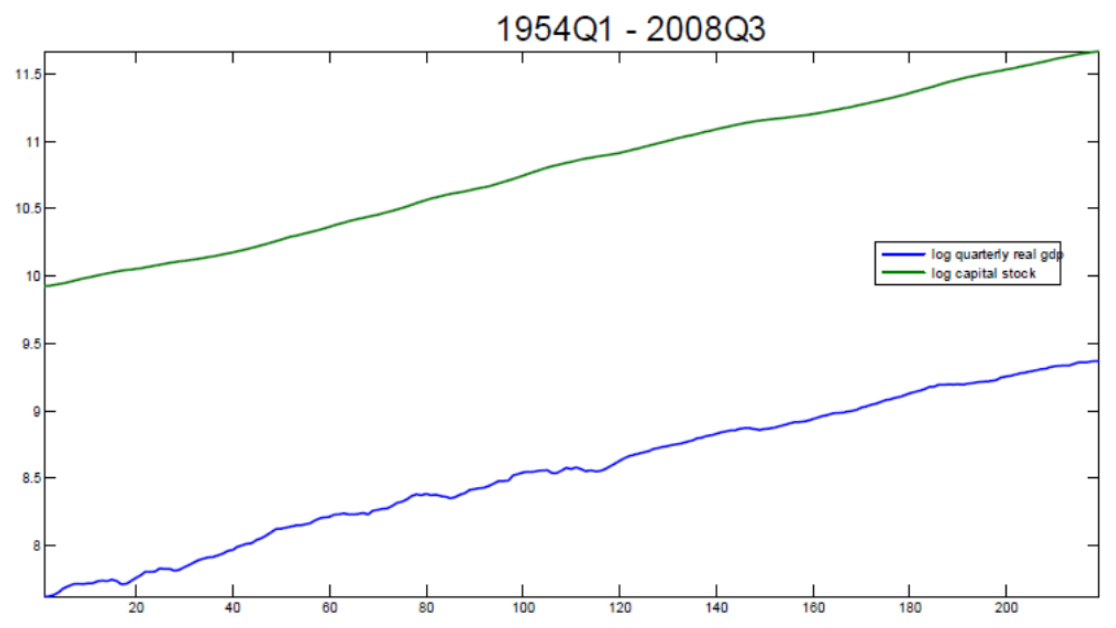
\includegraphics[width=0.92\textwidth]{topic1_figs_BC/capital_vs_gdp.png}
\end{center}
\end{frame}

\begin{frame}{Measuring the Solow residual (TFP)}
\label{slide:BC_SolowResidual}
\small
Gather data on \(\{Y_t,K_t,n_t\}\). With Cobb--Douglas production,
\[
Y_t = A_t K_t^{\alpha}(n_t X_t)^{1-\alpha}.
\]
Taking logs:
\[
\log A_t = \log Y_t - \alpha\log K_t - (1-\alpha)\log n_t - (1-\alpha)\log X_t.
\]
Decompose \(A_t\) into deterministic growth and stationary technology:
\[
A_t = z_t X_t^{1-\alpha},\qquad \frac{X_{t+1}}{X_t}=\gamma_x.
\]
Then a common specification is an AR(1) for the stationary component:
\[
\log z_{t+1}=\rho\log z_t + \varepsilon_{t+1},\qquad \varepsilon_t\sim \mathcal{N}(0,\sigma_\varepsilon^2).
\]
Estimating \((\rho,\sigma_\varepsilon)\) pins down the persistence and variance of technology shocks.
\end{frame}

\begin{frame}{Solow residual plot (illustration)}
\label{slide:BC_SolowPlot}
\small
\begin{center}
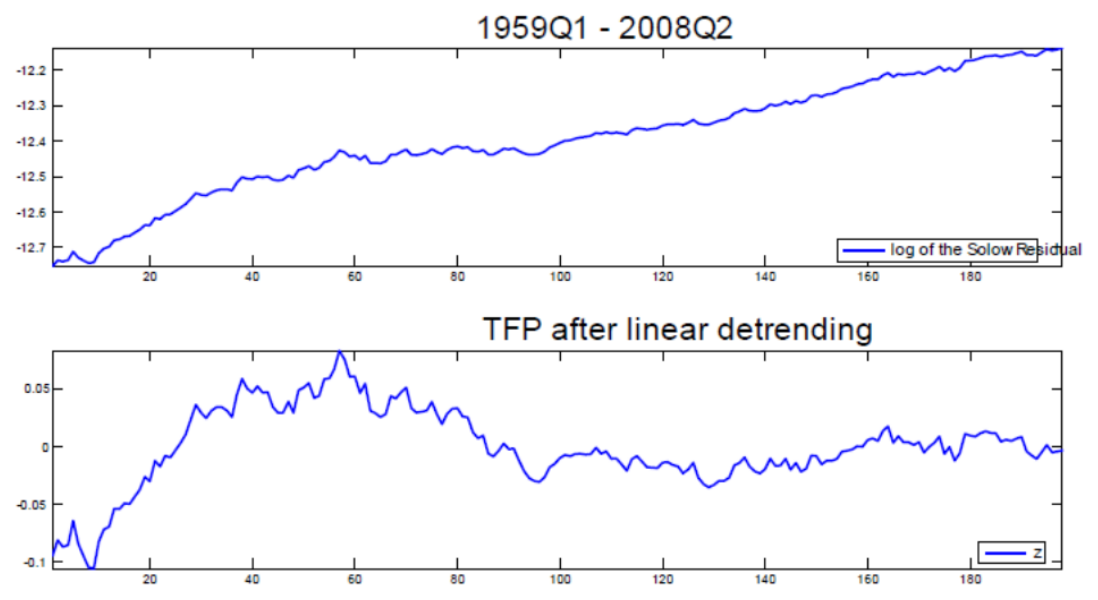
\includegraphics[width=0.92\textwidth]{topic1_figs_BC/solow_residual.png}
\end{center}
\end{frame}

\begin{frame}{Wrap-up: RBC pipeline}
\label{slide:BC_Wrap}
\small
\begin{itemize}
    \item Start with the benchmark RBC model (household + firm + markets).
    \item Introduce growth (labor-augmenting \(X_t\)) \(\Rightarrow\) BGP rather than steady state.
    \item Growth-deflate to get a stationary problem in efficiency units.
    \item Measure \(K_t\) and \(z_t\) from data (perpetual inventory, Solow residual).
    \item Use calibrated parameters and estimated shocks to study business-cycle dynamics.
\end{itemize}
\end{frame}

\end{document}
